% !TEX root = ../lectures_olympics.tex

\chapter{量子物理初步}
到十九世纪末人们经过二百多年的努力,在牛顿力学的基础上又发展出了热力学和电磁学,到二十世纪初的人们普遍认为,物理学的大厦已经接近完成,剩下的只需要对理论的细节稍做修补,多测量几个有效数字而已,除了两个问题,也就是著名的两朵乌云:一是迈克尔逊-莫雷实验,另外一个则是对黑体辐射光谱测量。
在迈克尔逊-莫雷实验的基础上我们知道最终发展出了狭义相对论,极大地改变了我们对于时空的认识。
令人没有想到的是从黑体辐射光谱出发的研究竟然打开了一道认识微观世界的大门,完全改变了我们对于自然界的基本组成和相互作用的认识,在此基础上发展出的量子力学为最终认识自然的终级运动规律指明了道路。
下面我们就来重温这段历史。

\section{黑体辐射:能量的量子化}
所谓黑体是这样一种理想化的物质:它能够完全吸收照射在它上面的电磁辐射,而不会以入射光产生透射和反射。
它虽然不反射电磁波,但是会通过自发地发射电磁波而维持平衡。
所有照射在它上面的光,也就是能量会使它的温度升高,黑体辐射的电磁波的能量与它的温度有关,温度越高发射功率就越大,理论和实验均表明,黑体表面单位面积辐射功率与它温度的四次方成正比:
\begin{equation}
P=\sigma T^4
\end{equation}
这就是著名的斯特潘-玻尔兹曼定律,式中的比例常数就是斯特藩-玻尔兹曼常数。
当入射和发射功率相等时黑体将处于热平衡状态。


黑体辐射的光谱与黑体的材料、大小或其它物理量均无关,只与处于热平衡状态黑体的温度有关。
理论计算和实验观测均表明黑体辐射包含所有的频率,辐射光的能量在不同频率之间并不是平均分布,而是具有如下图所示的形状。
对于任何一个给定的温度$T$,都有一个给定的波长$\lambda_{max}$,在此波长处的辐射功率为最大值,也就是辐射曲线的最高点,不同温度的功率最大值所对应的波长和温度有简单的关系:
\begin{equation}
\lambda_{max}\cdot T = \text{常数}
\end{equation}
这就是著名的维恩位移定律,其中的常数对于所有的黑体均一致。
\begin{figure}
\centering
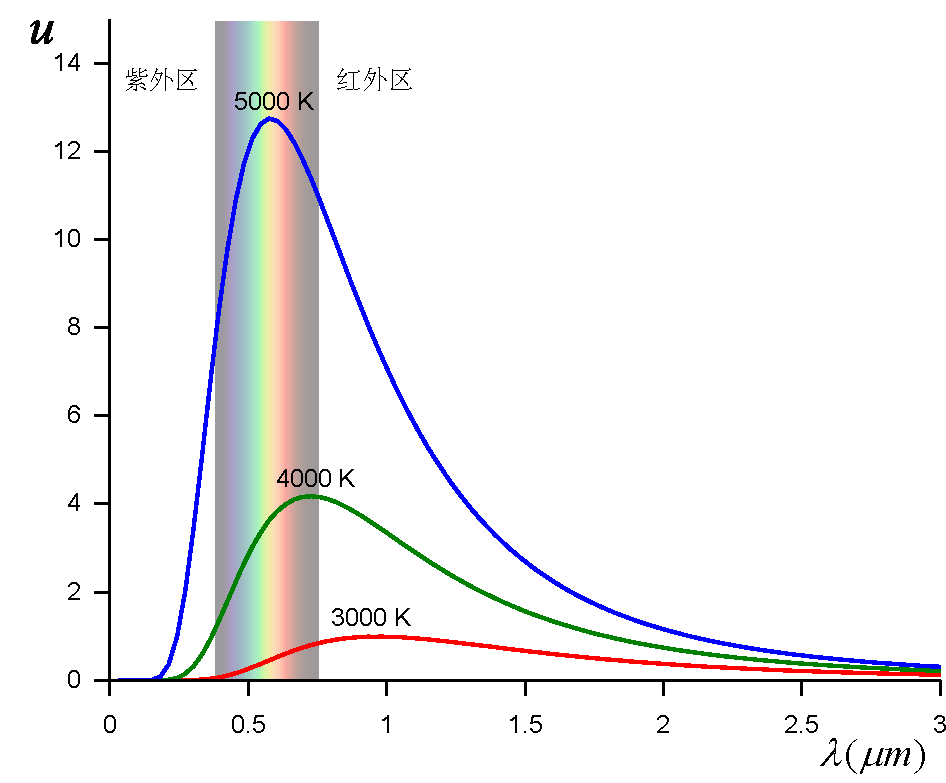
\includegraphics[width=0.6\linewidth]{images/particle-5}
\caption{黑体辐射能量密度与波长的关系,不同的温度有不同的辐射光谱}
\label{fig:particle-5}
\end{figure}

同时考虑黑体辐射的斯特潘-玻尔兹曼定律和维恩位移定律可以得出一个结论,黑体辐射的光谱必须具有
\begin{equation}\label{eqn: 近代物理,黑体辐射一般形式}
u=u(\nu,T)= \nu^3f(\frac{\nu}{T})
\end{equation}
其中$\nu$为辐射光的频率,它与波长的关系为$\lambda\nu=c$,$f$为某一给定的函数。
函数$f(\frac{\nu}{T})$的具体形式可由实验结果拟合而得到,但人们更感兴趣的是如何从理论上得到它的形式。
为此需要对黑体辐射的本质做出一些假设,通过理论计算而得到。

一种观点是黑体辐射是由处于热平衡状态的黑体空腔当中的电磁场所给出,电磁波在单位体积内在频率$\nu$到$\nu+\Delta\nu$范围内的数密度由
\begin{equation}
\frac{4\pi\nu^2}{c^3}\Delta\nu
\end{equation}
所给出,而热平衡时每个自由度都会平均地分配能量$\frac{1}{2}kT$,考虑到振子的能量为”动能“和”势能“构成以及光有两个偏振模式空腔辐射的功率密度可以写为
\begin{equation}
u(\nu,T)=\frac{8\pi\nu^2}{c^3}kT
\end{equation}
这就是著名的瑞利-金斯辐射公式。
它与实验测量到的黑体辐射谱在低频端吻合地非常之好,但是在高频端严重偏离,并且因为频率越高振子的数密度越大,导致总的辐射功率在高频处趋于无穷,历史上称这个结论为紫外灾难。

为了避免此外灾难,假设黑体辐射具有类似气体分子的性质,与气体分子速度分布函数做类比并考虑到黑体辐射的两个性质,维恩给出了一个黑体辐射公式,他把\ref{eqn: 近代物理,黑体辐射一般形式}中的函数$f(\frac{\nu}{T})$取成指数函数并配以合适的系数得到著名的维恩曲线:
\begin{equation}
u(\nu,T)=a\nu^3e^{-b\frac{\nu}{T}}
\end{equation}
其中$a$、$b$为两个未知系数,原则上可由实验所给出。
与黑体辐射曲线相比,在高频端维恩公式吻合得非常理想,但是在低频部分维恩曲线会得出荒谬的结果:对于极高的温度上式变成了
\begin{equation}
\lim_{T\rightarrow\infty}u(\nu,T)=a\nu^3
\end{equation}
黑体辐射的能量将会无限增加,这就是所谓的红外灾难。
\begin{figure}
\centering
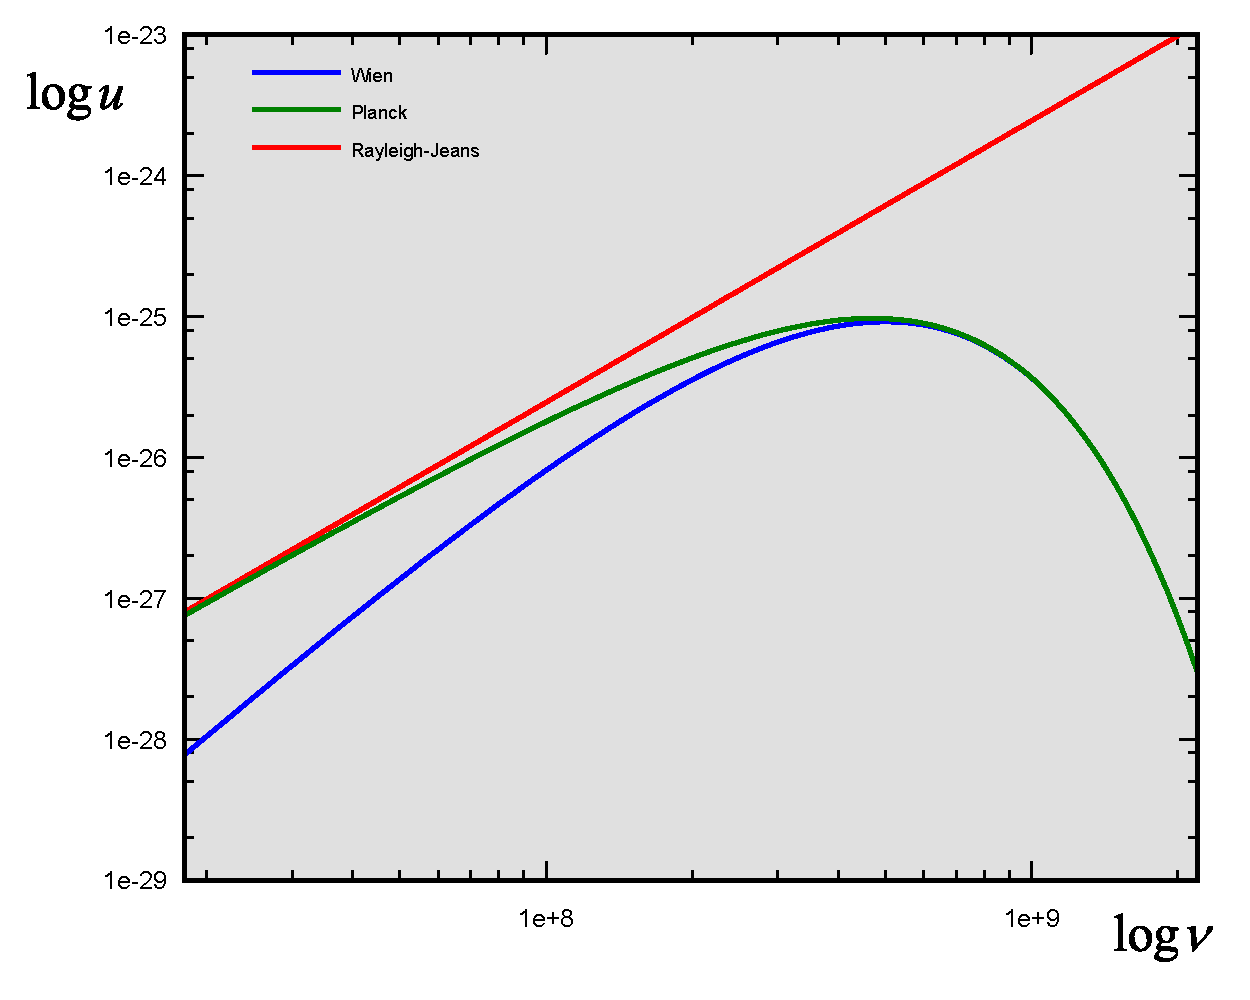
\includegraphics[width=0.6\linewidth]{images/particle-6}
\caption{瑞利-金斯曲线和维恩曲线与实验值的偏离,各个量用对数标出,从上至下三条线分别为瑞利-金斯曲线、实验曲线和维恩曲线}
\label{fig:particle-6}
\end{figure}

为了得到正确的黑体辐射公式,普朗克从热力学出发,坚持认为当时刚刚发现的物理量--熵是一个描写热平衡状态物体基本的物理量\footnote{这一点在当时其实是有争议的},黑体在热平衡时瑞利-金斯公式和维恩公式同时贡献热力学系统的统计涨落,利用插值法得出了著名的普郞克黑体辐射公式:
\begin{equation}
u(\nu,T)=\frac{8\pi\nu^3}{c^3}\frac{1}{e^{\frac{h\nu}{kT}}-1}
\end{equation}
其中$T$为黑体的温度,$k$为玻尔兹曼常数,$h$为一个新的常数,后来被称做普郎克常数,它是量子力学中最基本的物理量,今后当任何一个物理公式中出现了朗克常数$h$时,它一定是量子力学的结论。
普朗克辐射公式无论在红外还是紫外端都与实验曲线吻合。

得到满足实验的辐射公式以后,普朗克继续寻找能够导致该公式的微观机制,最后的结果令人大吃一惊:对于任意给定的频率的辐射,能量并不是连续地接收和发射,单次的吸收或发射的能量必须是普朗克常数$h$和辐射频率$\nu$乘积的整数倍:
\begin{equation}
\Delta E = n\cdot h\nu
\end{equation}
其中$n$为任意的整数!
这告诉我们微观世界的能量传递和转化并不是连续发生的,每个微观过程吸收或放出的能量是由“能量量子”的传递而完成。



%%%%%%%%%%%%%%%%%%%%%%%%%%%%%%%%%%
\begin{example}
在粗略的近似下认为太阳系中所有天体均为黑体,试论证行星的温度与其本身的半径无关,与它到太阳的距离成反比。
\tagged{student}{\vspace*{4cm}}
\begin{taggedblock}{teacher}
\noindent
解析:
\[
P_吸 \propto \frac 1 {R^2} \pi r^2
\]
\[
P_放 \propto \sigma T^4 \cdot 4 \pi r^2
\]
所以

\[
T^4 \propto \frac 1 {R^2}
\]
\end{taggedblock}
\end{example}
%%%%%%%%%%%%%%%%%%%%%%%%%%
%
%%%%%%%%%%%%%%%%%%%%%%%%%%%%%%%%%%
\begin{example}
地球的平均温度为$T = 287\unit{K}$。
如果地球到太阳的平均距离减小$1\%$的话新的平均温度为多少?
\tagged{student}{\vspace*{4cm}}
\begin{taggedblock}{teacher}
\noindent
解析:
288.4 K
\end{taggedblock}
\end{example}
%%%%%%%%%%%%%%%%%%%%%%%%%%


%%%%%%%%%%%%%%%%%
\begin{example}
在地面上方垂直于太阳光的入射方向,放置一半径$R=0.10\unit{m}$、焦距$f=0.50\unit{m}$的薄凸透镜,在薄透镜下方的焦面上放置一黑色薄圆盘(圆盘中心与透镜焦点重合),于是可以在黑色圆盘上形成太阳的像。
已知黑色圆盘的半径是太阳像的半径的两倍。圆盘的导热性极好,圆盘与地面之间的距离较大。
设太阳向外辐射的能量遵从斯特藩—玻尔兹曼定律:在单位时间内在其单位表面积上向外辐射的能量为$W = \sigma T^4$,式中$\sigma$为斯特藩—玻尔兹曼常量,$T$为辐射体表面的的绝对温度。
对太而言,取其温度$t_S = 5500^\circ C$。
大气对太阳能的吸收率为$\alpha = 0.40$。
又设黑色圆盘对射到其上的太阳能全部吸收,同时圆盘也按斯特藩—玻尔兹曼定律向外辐射能量。
如果不考虑空气的对流,也不考虑杂散光的影响,试问薄圆盘到达稳定状态时可能达到的最高温度为多少摄氏度?

\tagged{student}{\vspace*{4cm}}
\begin{taggedblock}{teacher}
\noindent
解析:25-2. 根据能量的关系可知
\[
\frac{\sigma T_S^4 4\pi R_S^2}{4\pi r_E^2}\pi R^2(1-\alpha) = \sigma T^4 2 \pi r^2,
\]
其中$R_S$为太阳半径,$r_E$是地球轨道半径,$R$是透镜半径,$r$为黑板半径,注意黑板上、下表面均会辐射热量。
有几个未知数可以通过已知条件消去,考虑太阳边缘通过透镜中点的光线,它们都是直线传播,我们有
\[
\frac{f}{r_E} = \frac{r_I}{R_S}
\]
其中$r_I$是太阳像的半径,根据假设它等于$r/2$,这样刚刚好把所有的未知量全部消去,可得
\[
T^4 = \frac{(1-\alpha)R^2}{8r^2}T_S^4
\]
代入数字可得最终结果$T = 1.4\pow{3}\unit{K}$。
\end{taggedblock}
\end{example}
%%%%%%%%%%%%%%%%%%%%%%

%%%%%%%%%%%%%%%%%%%%%%%%%%%%%%%%%%
\begin{example}
有两个相对放置、彼此平行的黑体表面,温度分别为$T_h$和$T_l$,它们与热源接触保持恒温,中间为真空。

为了降低两表面之间辐射热流,可在中间真空区域放置一个由两个彼此隔离的黑体板构成的热屏幕装置,与两个恒温表面无热接触。
经过一段时间以后形成稳定的平衡状态,求插入隔热板后两个黑体表面之间的热流与插入之前的比值。
\\
\\
\tagged{student}{\vspace*{4cm}}
\begin{taggedblock}{teacher}
\noindent
解析:$\frac{1}{3}$,只需根据黑体辐射的性质以及平衡的条件即可得到结果。
\end{taggedblock}
\end{example}
%%%%%%%%%%%%%%%%%%%%%%%%%%




















\section{光量子假设:光电效应,辐射(物质)的量子化}
在普朗克发现的基础上爱因斯坦进一步指出,处于空腔之中的电磁波在频率很高时,它们的热力学性质和气体分子或其它粒子构成的热力学系统有着相似之处,尤其是熵这样一个物理量。
经过计算他发现,一个包含有频率相同的高频辐射的空腔的熵与包含有
\begin{equation}
N=\frac{E}{h\nu}
\end{equation}
个分子的气体的熵惊人地一致,其中$E$为包含高频单色光的空腔的总能量,而$\nu$则是光的频率,另外$h$就是普朗克常数。
这就意味着光在某种情况下并不像在经典力学那样是由连续的电磁波构成,而是由为数众多、不可分割的光量子所组成,每个光量子的能量与光的频率有关:
\begin{equation}
E=h\nu
\end{equation}
这就是著名的爱因斯坦的光量子理论\footnote{需要特别指出的是虽然爱因斯坦的相对论影响更为深远,但他并未由此拿到诺贝尔奖,反而是由于光量子假说获得了1921年的诺贝尔奖}。
因为光子静止质量为零,上式与相对论结合还能够得出具有给定频率光子的动量
\begin{equation}
p = \frac{E}{c} = \frac{h\nu}{c} = \frac{h}{\lambda},
\end{equation}
其中$\lambda$为光子的波长。


\begin{figure}[ht]
\centering
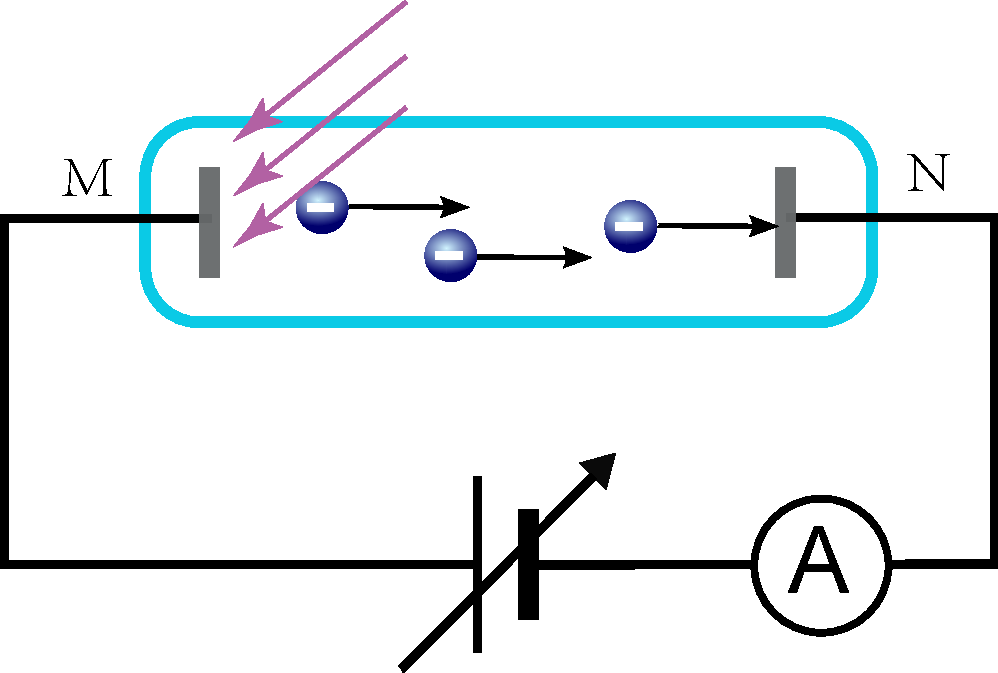
\includegraphics[width=0.6\linewidth]{images/particle-8}
\caption{光电效应}
\label{fig:particle-8}
\end{figure}

由光量子理论可以得到很多结论,它们无一例外地都与实验吻合。
这其中最为重要的当属光量子理论对光电效应的解释。
实验表明某些物质在光照下会有电子发射出来,这种现象称之为\emph{光电效应}。
图\ref{fig:particle-8}是用来研究光电效应的一个实验装置,其中$M$为光电管的阴极,它能够在光照下发射光电子,这些光电子被阳极$N$所接收,这样回路中将进行一个电流,称为\emph{光电流}。
利用一个可变电动势的电源可以对光电流进行控制。
通过改变入射光的强度、频率以及反射电压的大小,人们发现光电效应满足以下规律:
\begin{enumerate}
\item 光电流几乎在光照的瞬间就会产生,而当光照消失以后光电流也几乎瞬间消失,响应的时间差小于$10^{-9}\unit{s}$;
\item 逐渐调节可变电电源,使$N$的电势高于阴极$M$,起初光电流增加,但当电压增加到某一值后光电流大小保持不变,要想继续提高光电流强度必须增加入射光的强度。
\item 逸出电子的动能有一最大值$E_m = \frac{1}{2}m_ev_m^2$,当在回路中加的反向电压时有一最大值$U_m$,它满足
\begin{equation}
eU_m = \frac{1}{2}m_ev_m^2 = E_m
\end{equation}
当$U>U_m$时,无论如何提高入射光强度均无法产生光电流。
$U_m$称为反向截止电压。
\item 不同材料都有一个能够产生光电效应的最小入射光频率$\nu_0$,只有入射光频率$\nu>\nu_0$才能够发生光电效应。
更精确的测量则给出入射光频率$\nu$,最小入射光频率$\nu_0$与出射光电子最大动能$E_m$的关系为
\begin{equation}
h\nu-h\nu_0 = E_m = eU_m.
\end{equation}
\end{enumerate}

%%%%%%%%%%%%%%%%%
\begin{example}

试根据光量子假说解释光电效应的实验现象
\tagged{student}{\vspace*{4cm}}
\begin{taggedblock}{teacher}

解析:略
\end{taggedblock}
\end{example}
%%%%%%%%%%%%%%%%%%%%%%


%%%%%%%%%%%%%%%%%
\begin{example}

已知某个平面镜反射的光能量为入射光能量的$80 \%$。
试判断下列说法是否正确,并简述理由。

1. 反射光子数为入射光子数的$80  \%$;


2.每个反射光子的能量是入射光子能量的$80 \%$。


\tagged{student}{\vspace*{2cm}}
\begin{taggedblock}{teacher}

解析:根据光量子假设,1是对的,2是错的,光反射时不会改变频率
\end{taggedblock}
\end{example}
%%%%%%%%%%%%%%%%%%%%%%


%%%%%%%%%%%%%%%%%
\begin{example}

波长为$350\unit{nm}$的光波入射到某光电材料表面,能量最高的光电子在$1.5\pow{-5}\unit{T}$的磁沿半径为$18.0\unit{cm}$的圆轨道运动。
试求该光电材料的逸出功。
\tagged{student}{\vspace*{4cm}}
\begin{taggedblock}{teacher}

解析:直接根据已知条件计算即可
\[
W_0 = \frac{hc}{\lambda}-\frac{e^2B^2R^2}{2m} = 2.9\unit{eV}.
\]
\end{taggedblock}
\end{example}
%%%%%%%%%%%%%%%%%%%%%%





%%%%%%%%%%%%%%%%%
\begin{example}

某金属材料发生光电效应的最大波长为$\lambda_0$,将此材料制成一半径为$R$的圆球,并用绝缘线悬挂于真空室内.若以波长为$\lambda(\lambda<\lambda_0)$的单色光持续照射此金属球,该金属球发生光电效应所产生光电子的最大初动能为\kong\kong ,此金属球可带的电荷量最多为\kong\kong 。
\tagged{student}{\vspace*{2cm}}
\begin{taggedblock}{teacher}

解析:$\frac{hc(\lambda_0-\lambda)}{\lambda_0\lambda}$, $\frac{hcR(\lambda_0-\lambda)}{ke\lambda_0\lambda}$。

球不带电时电子最容易跑出,根据已知信息可知电子溢出功为$\frac{hc}{\lambda_0}$,在受光照射时电子的动能满足
\[
\frac{hc}{\lambda} = \frac{hc}{\lambda_0}+\frac{kQe}{R}+E_k
\]
从中可看出$Q$越小电子动能越大,所以电子最大动能$\frac{hc(\lambda_0-\lambda)}{\lambda_0\lambda}$。
当带电太多以后就无法发生光电效应,简单计算表明最大带电量$\frac{hcR(\lambda_0-\lambda)}{ke\lambda_0\lambda}.$
\end{taggedblock}
\end{example}
%%%%%%%%%%%%%%%%%%%%%%



%%%%%%%%%%%%%%%%%
\begin{example}
入射光以入射角$i$射到一不透光的表面上,入射光的能流密度为$I$。
设表面对光的能量反射率为$R$,试求该表面单位面积所受的光压和切向力。
\begin{flushright}
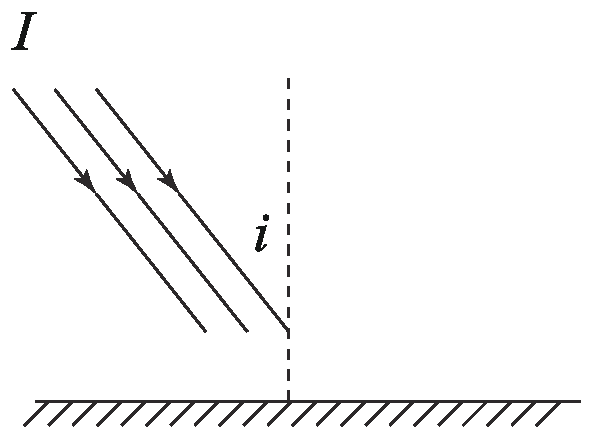
\includegraphics[width = 0.3\textwidth]{images/particle-11.pdf} 
\end{flushright}

\tagged{student}{\vspace*{3cm}}
\begin{taggedblock}{teacher}

解析:对单个光子的运动分析,光子分两种,一种是被吸收的,一种是被反射的,动量变化不尽相同。
最简单的假设下,入射光是单色光,波长为$\lambda$,这样单位时间里的光子数
\[
n = \frac{I}{hc/\lambda}.
\]
直接计算可得法向力
\[
N = \frac{I}{C}(1+R)\cos i,
\]
切向力
\[
T = \frac{I}{c}(1-R)\cos i\sin i
\]
\end{taggedblock}
\end{example}
%%%%%%%%%%%%%%%%%%%%%%


%%%%%%%%%%%%%%%%%
\begin{example}

试从相对论能量和动量的角度分析论证 

1. 一个光子与真空中处于静止状态的自由电子碰碰撞时,光子的能量不可能完全被电子吸收。

2. 光子射到金属表面时,其能量有可能完全被吸收被使电子逸出金属表面,产生光电效应。 

\tagged{student}{\vspace*{4cm}}
\begin{taggedblock}{teacher}

解析:动量守恒、能量守恒方程联立,无论用经典的或相对论性的方程,都会得到不合常理的结果。
\end{taggedblock}
\end{example}
%%%%%%%%%%%%%%%%%%%%%%

%%%%%%%%%%%%%%%%%%%%%%%%%%%%%%%%%%
\begin{example}
一个波长为$ \lambda$的光子与一个静止的电子发生弹性碰撞。
碰撞之后电子获得的速度远远小于光速,求出射方向与入射方向夹角为$\theta$的光子的波长$\lambda'$。
结果用出射角度$\theta$、电子质量$m_e$和普朗克常数$h$表示。
\begin{flushright}
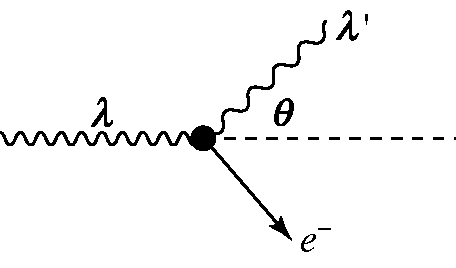
\includegraphics[width=0.4\textwidth]{images/particle-1.pdf}
\end{flushright}
\tagged{student}{\vspace*{4cm}}
\begin{taggedblock}{teacher}

解析:
\[
\lambda '=\frac{\frac{hc}{\lambda}(1-\cos\theta)+m_0 c^2}{m_0 c^2}\lambda
\]
\end{taggedblock}
\end{example}
%%%%%%%%%%%%%%%%%%%%%%%%%%


%%%%%%%%%%%%%%%%%
\begin{example}
如图所示,在真空中有一个折射率为$n$($n>n_0$,$n_0$为真空的折射率)、半径为$r$的质地均匀的小球。
频率为$\nu$的细激光束在真空中沿直线$BC$传播,直线$BC$与小球球心$O$的距离为$l(l<r)$,光束于小球体表面的点$C$点经折射进入小球(小球成为光传播的介质),并于小球表面的点$D$点又经折射进入真空。
设激光束的频率在上述两次折射后保持不变,求在两次折射过程中激光束中一个光子对小球作用的平均力的大小。
\begin{flushright}
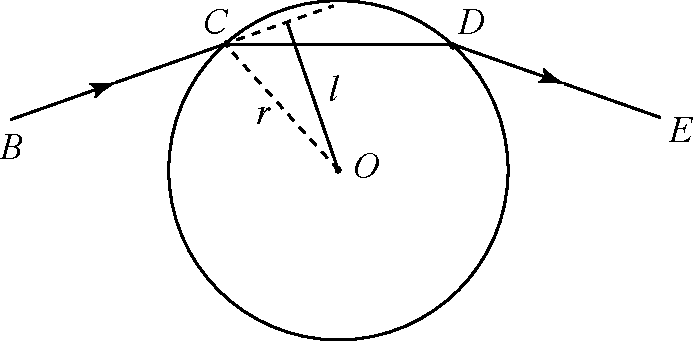
\includegraphics[width=0.4\textwidth]{images/particle-2.pdf}
\end{flushright}

\tagged{student}{\vspace*{4cm}}
\begin{taggedblock}{teacher}

解析:17届复赛-2
\end{taggedblock}
\end{example}
%%%%%%%%%%%%%%%%%%%%%%

%%%%%%%%%%%%%%%%%
\begin{example}
光在物体表面反射或者被吸收时,光子将其动量传给物体,使光具有对物体的辐射压力(光压)。
利用光压,可实现对某些微小粒子的精确操控(光摄)。
设在$y\ge L$的区域有一匀强激光场,沿$z$轴负方向入射,其强度(单位时间内通过单位横截面积的光能)为$I$;在$y\in (-L,L)$之间没有光场,其横截面如图所示。
一密度为$\rho$的三棱柱形小物体(其横截面是底边长为$2L$、底角为$\theta$的等腰三角形)被置于光滑的水平面$xy$上,其朝上的$A$和$B$两面均涂有特殊反射层,能完全反射入射光。
小物体初始时静止,位置如图。

1. 假定光子的反射角等于入射角,且反射前后光子的频率不变.试求:

(a)小物体在受到激光场照射后的动力学方程;

(b)小物体从初始位置向$y$轴负方向移动$3L/2$的距离所需的时间。

2. 实际上,由于小物体的运动,反射光子频率会有微小的变化;在小物体从初始位置向$y$轴负方向移动到距离$3L/2$的过程中,定性比较反射光子与入射光子频率的大小及其随时间的变化。
\begin{flushright}
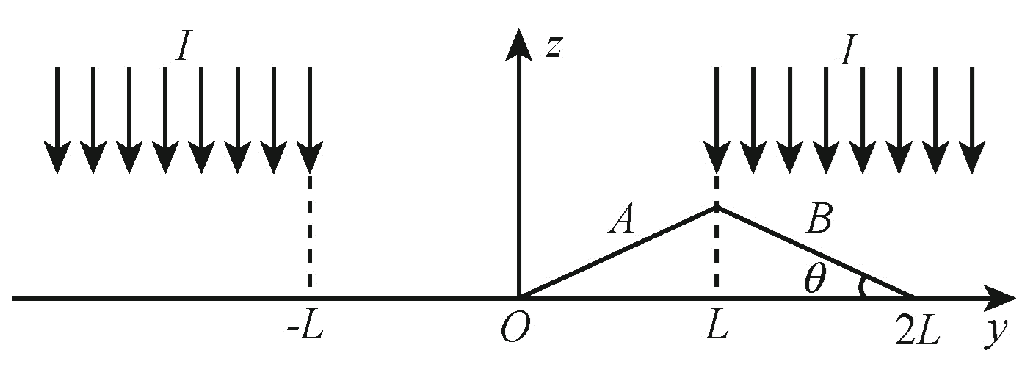
\includegraphics[width = 0.5\textwidth]{images/particle-3.pdf} 
\end{flushright}


\tagged{student}{\vspace*{4cm}}
\begin{taggedblock}{teacher}

解析:32届决赛-4
\end{taggedblock}
\end{example}
%%%%%%%%%%%%%%%%%%%%%%




\section{氢原子光谱:轨道(运动)的量子化}
不仅在黑体辐射和诸如光电效应的现象中发现了自然界中的不连续现象,对原子光谱的观测也发现原子发出的光的频率并不是连续的,只会发出一些特定波长或频率的光,图\ref{fig:particle-12}就是氢原子光谱的可见光部分。
对于氢原子来说,它所有的谱线能够总结为
\begin{equation}
\nu = R_E(\frac{1}{m^2}-\frac{1}{n^2})
\end{equation}
其中$R_E = 1.0967758\pow{7}\unit{m^{-1}}$称为里德伯恒,为一常数,而$m$、$n$则是任意的整数。

\begin{figure}[ht]
\centering

\includegraphics[width=0.7\linewidth]{images/particle-12}
\caption{氢的可见光光谱}
\label{fig:particle-12}
\end{figure}


原子当中的这些光是如何发出的成为摆在当时人们面前的一道难题。
从$\alpha$粒子的散射实验已知,原子是由位于中心质量很大但又体积很小的原子核以及在核外运动的电子构成。
根据传统的电磁学,电子将在原子核的库仑力作用下做椭圆轨道运动,但是如果这幅图像成立的话,电子的加速度时刻不为零,根据电磁学做加速运动的电子将会辐射电磁波,这样电子的能量将不断地被电磁波带走而损失,最终坠向原子核,不会形成稳定的原子,这与观测现象明显矛盾。
为了从理论上得到稳定的原子就必须对电子围绕原子核的运动做出一些不同于经典电磁学的假设。

\begin{figure}[!b]
\centering
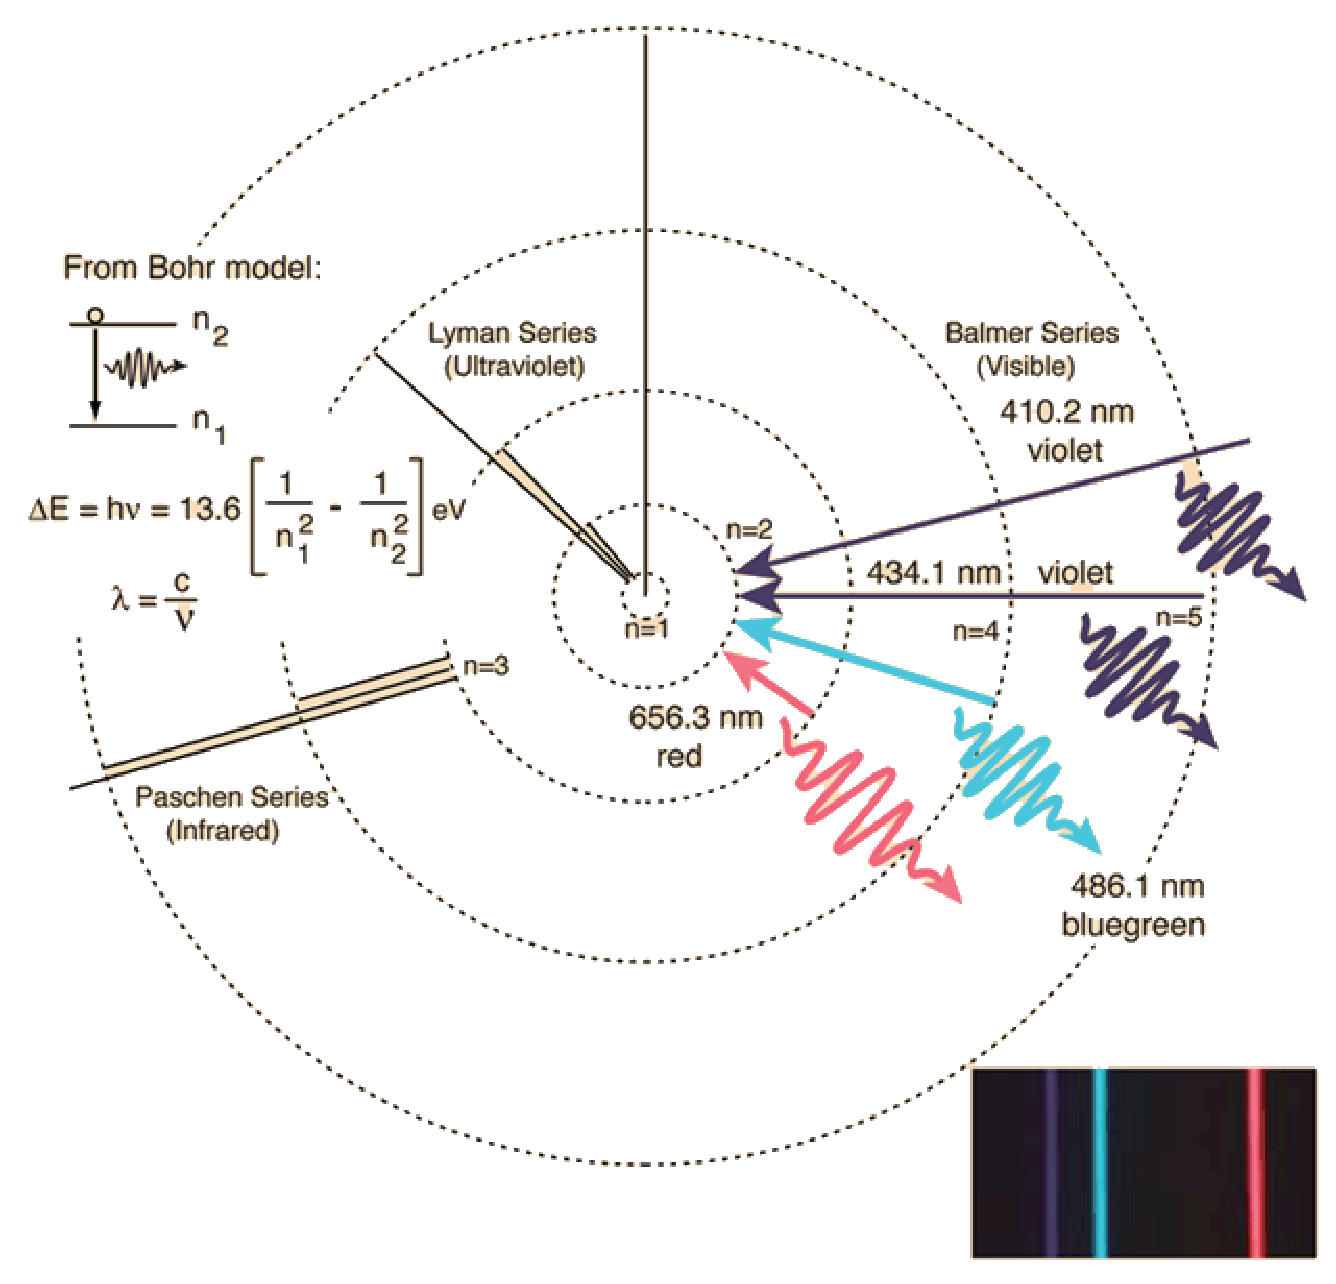
\includegraphics[width=0.5\linewidth]{images/particle-13}
\caption{玻尔氢原子模型}
\label{fig:particle-13}
\end{figure}

基于实验现象,丹麦物理学家玻尔对原子的外层电子的运动做出如下假设:
\begin{description}
\item[稳定能级] 电子会在一些用整数标记的稳定轨道上运动,并且在运动过程中并不会辐射电磁波而损失能量。由某一整数$n$标记的轨道称做电子的一个能级,处于能级$n$上的电子具有能量$E(n)$。
\item [光量子吸收和发射]同时电子有可能在不同的轨道之间变化,这种变化被称做跃迁,跃迁过程中会吸收或发射光子,光子的频率由两个能级的能量差决定:
\begin{equation}
hv_{m\rightarrow n}=E(m)-E(n)
\end{equation}
当能级$m$的能量大于能级$n$时原子将会向外发射光子,反之为吸收。
\item[对应原理] 当$n$为很大的整数时,电子辐射光子的频率与经典力学所给出的结果一致。
也就是说当$n$趋于无限大时,电子在能级之间跃迁所发出光的频率为在与相同能量$E(n)$运动的频率的整数倍。
将对应原理应于于氢原子,电子的轨道角动量必须为约化普朗克常数$\hbar$的整数倍:
\begin{equation}\label{eqn: 近代物理,玻尔轨道条件}
L_n = m_evr = n\cdot\hbar=n\cdot\frac{h}{2\pi}
\end{equation}
这就是著名的原子玻尔模型。
\end{description}





\begin{example}
试根据玻尔轨道的条件\ref{eqn: 近代物理,玻尔轨道条件}证明对于由整数$n$所给出的氢原子能级的半径$r(n)$和能量$E(n)$分别是
\begin{equation}
r(n)=\frac{\varepsilon_0 h^2}{\pi m_ee^2}\cdot n^2,\qquad E(n)=-\frac{m_ee^4}{8\varepsilon_0^2h^2}\cdot\frac{1}{n^2}
\end{equation}
\exspace{4}
\end{example}



%%%%%%%%%%%%%%%%%
\begin{example}
氢原子基态轨道半径$a_0 = 0.0529\unit{nm}$(玻尔半径)。
$\mu-$氢原子是普通氢原子中的电子被$\mu$子代替的产物,已知$\mu$子和电子电量相同,但质量是电子的207倍,如果依然假设质子的质量远大于$\mu$子质量,求$\mu-$氢原子的基态半径。

\tagged{student}{\vspace*{4cm}}
\begin{taggedblock}{teacher}

解析:$2.56 \pow{-4} nm$
\end{taggedblock}
\end{example}
%%%%%%%%%%%%%%%%%%%%%%




%%%%%%%%%%%%%%%%%
\begin{example}
某金属受到频率为$11.8\pow{14}\unit{Hz}$的紫外线照射时,测得其反向截止电压为$2.96\unit{V}$。
如果用氢气照射该金属,则在氢的发射光谱中哪些能级的跃迁可能使该金属释放电子?
释放电子的最大速度是多少?

\tagged{student}{\vspace*{4cm}}
\begin{taggedblock}{teacher}

解析:所有从激发态跃迁到基态的辐射,以及从第三激发态及以上激发态跃迁到第一激发态的辐射。电子的最大速度为$2\pow{6}$m/s
\end{taggedblock}
\end{example}
%%%%%%%%%%%%%%%%%%%%%%


\begin{example}
【课后思考】试求对应原理出发指导玻尔轨道条件\ref{eqn: 近代物理,玻尔轨道条件}。

\exspace{4}
\end{example}





\section{波粒二象性:通向微观世界的大门}
玻尔的原子模型当中稳定轨道条件\ref{eqn: 近代物理,玻尔轨道条件}能够改写为
\begin{equation}
\frac{h}{m_ev}=\frac{2\pi r}{n}
\end{equation}
根据量纲分析可以看出上式的左边具有长度的量纲,右边的分母为量子数为$n$的定态轨道半径,而分母不是别的,正是轨道的量子数。
也就是说上式右边就是轨道周长与量子数的比值。
对于这个式子有一个形象的理解:电子在量子态上的存在形式与一列驻波非常相似,该驻波的波长为普朗克常数与电子动量的比值,对于量子数为$n$的能级电子驻波的波数正是能级$n$。

法国物理学家德布罗意将这样的思想大胆地推广到一般的情况:不但原子当中的电子,以任意速度运动的任何粒子同样具有类似的波动性,其波长与原子当中一致,为普朗克常数与电子动量的比值:
\begin{equation}
\lambda = \frac{h}{p}=\frac{h}{mv}
\end{equation}
也就是说,运动着的微观粒子在某种程度上会表现出波动性,具有波的一般性质,尤其是会发生干涉和衍射现象。
这些波动的现象在随后的电子晶格散射实验中被发现。






%%%%%%%%%%%%%%%%%
\begin{example}

一对正、负电子可形成一种寿命比较短的称为电子偶素的新粒子。
电子偶素中的正电子与负电子都以速率$v$绕它们连线的中点做圆周运动,假定玻尔关于氢原子的理论可用于电子偶素,求电子偶素处在各定态时正负电子之间的距离$r_n$和能量$E_n$以及第一激发态与基态能量之差。

\tagged{student}{\vspace*{4cm}}
\begin{taggedblock}{teacher}

解析:
\[
r(n)=\frac{\varepsilon_0 h^2}{\pi m_ee^2}\cdot n^2,\qquad E(n)=-\frac{m_ee^4}{8\varepsilon_0^2h^2}\cdot\frac{1}{n^2} ,\qquad 10.2eV
\]

\end{taggedblock}
\end{example}
%%%%%%%%%%%%%%%%%%%%%%



%%%%%%%%%%%%%%%%%
\begin{example}

由阴级$K$发射的电子(质量为$m$,电荷为$e$,设其初速度为零)经加速极$A$加速后垂直射向一开有两条平行狭缝的屏,电子自狭缝出射后打到一荧光屏上,如图所示。
由于电子具有波动性,荧光屏上将出现明暗相间的条纹。
设加速极$A$与阴极$K$之间的电压为$U$,两平行狭缝间的距离为$d$,试问:

1. 在整个装置的轴线与荧光屏的交点$O$处,将出现暗条纹还是亮条纹?

2. 设位于轴线外侧的第一条亮条纹出现在$\theta$角处,写出$\theta$的表示式,以$m,e,d,U$及其它有关常量表示。
\begin{flushright}
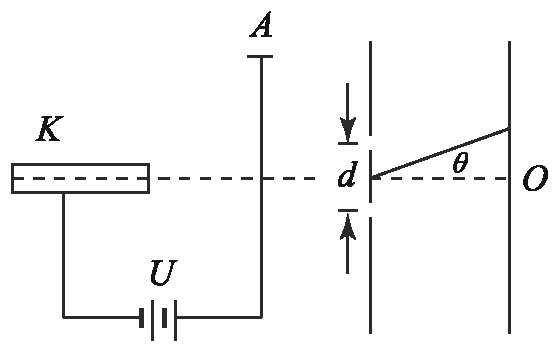
\includegraphics[width = 0.4\textwidth]{images/particle-4.pdf} 
\end{flushright}
\tagged{student}{\vspace*{1cm}}
\begin{taggedblock}{teacher}

解析:根据干涉规律,中间一定出现亮条纹。
电子的速度$v = \sqrt{\frac{2eU}{m}}$,这样电子的物质波长
\[
\lambda = \frac{h}{mv} = \frac{h}{\sqrt{2eUm}},
\]
所以第一级条纹$\theta = \frac{\lambda}{d} =\frac{h}{d\sqrt{2eUm}} $
\end{taggedblock}
\end{example}
%%%%%%%%%%%%%%%%%%%%%%


\section{量子力学,测不准原理}
黑体辐射、光电效应、氢原子轨道以及一系研究表明在原子尺度运动规律与经典的力学、电磁学有根本的不同,需要用新的物理来描写。
经过对实验现象的思考、与经典力学的比较人们最终建立了完整的量子力学体系,成为进一步认识微世界的理论基础。
量子力学与经典力学有着明显的区别,尤其是体现在对微观粒子运动的描写中。

经典力学认为我们可以以无限的精度测量一个质点的位置和速度,或者动量。
但是在量子力学中,由于所研究的对象就是自然界中那些最轻、最基本的粒子,测量的过程的本质是实验仪器、实验物质与基本粒子的相互作用过程,而任何试图对它们的测量必然会带来无法估计的影响。
这个对于粒子运动状态的不确定性由海森堡的\emph{测不准关系}给出,它表明对于任何一个给定的方向来说,建立一个沿此方向的坐标轴,其坐标用$x$来表示,这时对微观粒子在此方向上的位置$x$和动量$p_x = mv_x$\footnote{这里忽略相对论效应。}并不能够以任意的精度给出。
将位置$x$和动量$p_x$的不确定度记做$\Delta x,\Delta p_x$的话,它们之间必须满足
\begin{equation}
\Delta x\cdot\Delta p_x \ge h.
\end{equation}
如图\ref{fig:particle-7}所示,当试图精确测量其动量时,需要通过较长时间的测量来完成,那么位置的不确定性就会增加;反之如果将位置的测量变得很精确时,就必须用波长极小,或能量极高的光来确定它的位置,这时测量之后它和用来观测它的光子的碰撞之后会带来很大的动量不确定性。



\begin{figure}[ht]
\centering
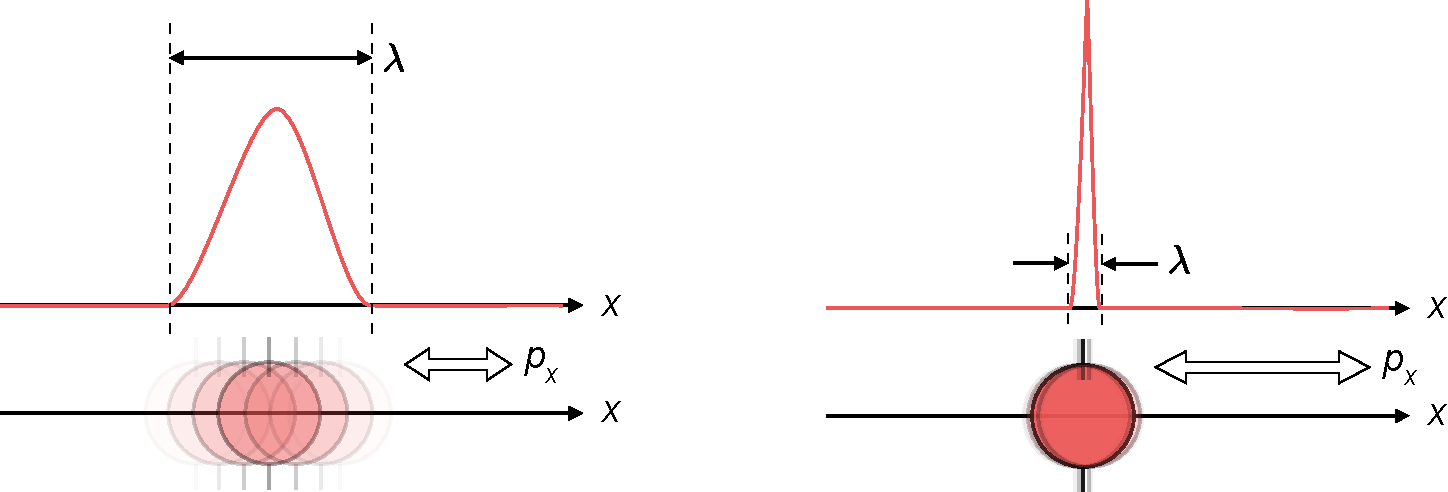
\includegraphics[width=0.6\linewidth]{images/particle-7}
\caption{测不准原理:在一特定方向上动量和位置的不确定性之间有反比关系}
\label{fig:particle-7}
\end{figure}




%%%%%%%%%%%%%%%%%
\begin{example}
有一个电子,已知它的德布罗意波是一列波长为$\lambda$,向$x$的正方向传播的平面波,它的动量$p_x$等于多少?它的坐标$x$如何?

\tagged{student}{\vspace*{2cm}}
\begin{taggedblock}{teacher}

解析:根据物质波理论,它的动量$p_x = h/\lambda$;因为动量完全已知,所以位置完全不能够确定。
\end{taggedblock}
\end{example}
%%%%%%%%%%%%%%%%%%%%%%



%%%%%%%%%%%%%%%%%
\begin{example}
一束电子以速度$v$沿$x$方向运动,在通过一个与运动方向垂直、宽度为$d$的狭缝之后继续飞行$L$撞向接收屏$MN$。
试分析电子在屏上垂直于初速度方向的分布情况。
\begin{flushright}
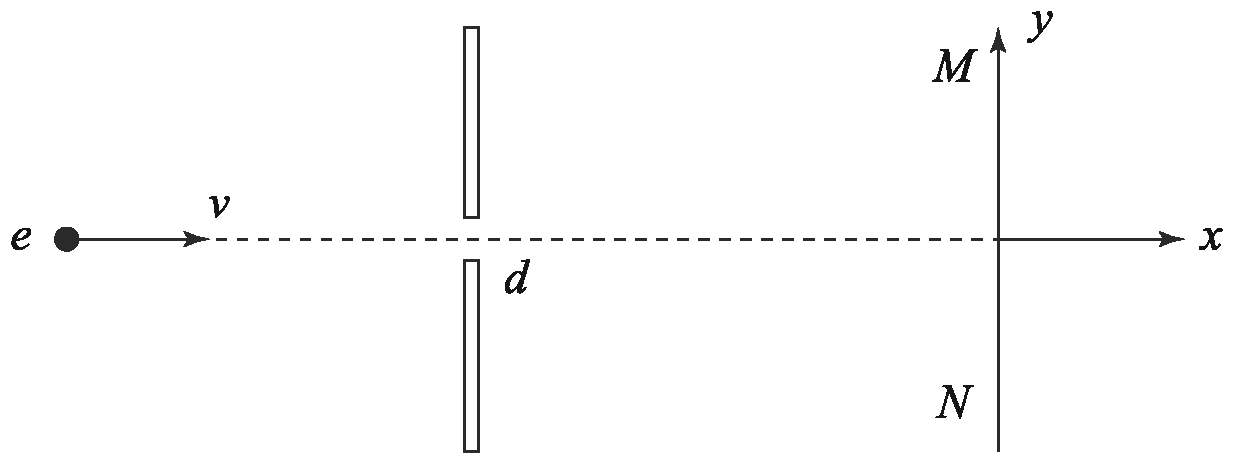
\includegraphics[width = 0.5\textwidth]{images/particle-9.pdf} 
\end{flushright}

\tagged{student}{\vspace*{3cm}}
\begin{taggedblock}{teacher}

解析:参考波长是$\frac{h}{mv}$的波的衍射
\end{taggedblock}
\end{example}
%%%%%%%%%%%%%%%%%%%%%%



%%%%%%%%%%%%%%%%%
\begin{example}
当对一个光子进行测量表明它存在于一个长度为$L$的波列当中,并且可以确定波列中有$N$个波峰,那么光的波长就是$L/N$,这是否意味着我们准确地测出了光子的动量了呢?
\begin{flushright}
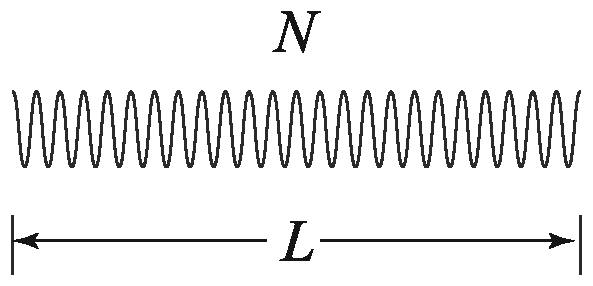
\includegraphics[width = 0.4\textwidth]{images/particle-10.pdf} 
\end{flushright}


\tagged{student}{\vspace*{4cm}}
\begin{taggedblock}{teacher}

解析:若波列长度确定,动量必然存在不确定性
\end{taggedblock}
\end{example}
%%%%%%%%%%%%%%%%%%%%%%

%%%%%%%%%%%%%%%%%
\begin{example}
【课后思考】设计尽可能多的试图同时测量微观粒子位置和动量的装置,再从微观粒子的相互作用出发分析测不准原理是如何工作的,你的装置为什么不能够同时测量位置和动量。

\tagged{student}{\vspace*{4cm}}
\begin{taggedblock}{teacher}

解析:
\end{taggedblock}
\end{example}
%%%%%%%%%%%%%%%%%%%%%%


